\section{Fluctuations, Criticality, and Geometric Response}
\label{sec:response}

\subsection{Critical Fluctuations and Divergent Response}

The geometric structures developed in the previous section are present in all thermodynamic systems. Under ordinary conditions, however, the associated response functions remain finite and the resulting geometry is comparatively benign. Critical phenomena provide a striking exception. Near a critical point, fluctuations become amplified, susceptibilities diverge, and characteristic length scales grow without bound. As a consequence, the geometric structures associated with thermodynamic response become increasingly pronounced and often dominate the observable behavior of the system.

From the perspective of response geometry, critical points represent regions where the metric sector becomes singular. The fluctuation-response relation implies that enhanced susceptibilities are accompanied by enhanced fluctuations, leading to large values of the thermodynamic metric. In this regime, neighboring thermodynamic states become increasingly distinguishable through their response, and geometric measures derived from fluctuations often exhibit universal scaling behavior.

The connection between criticality and geometry has a long history. Early work by Weinhold and Ruppeiner demonstrated that thermodynamic metrics provide a natural framework for characterizing fluctuations and stability near phase transitions. Subsequent studies showed that scalar curvature derived from these metrics often exhibits singular behavior at critical points and, in many systems, scales with the correlation volume. These observations established one of the earliest connections between geometric structure and collective thermodynamic behavior.

The geometric interpretation of criticality has subsequently expanded in several directions. Information-geometric approaches based on Fisher metrics have been used to characterize phase transitions through statistical distinguishability, while quantum geometric tensors and quantum Fisher information have provided analogous descriptions of quantum critical phenomena. Despite differences in mathematical formulation, these approaches share a common underlying principle: critical points correspond to regions where response becomes amplified, rendering geometric structures particularly prominent.

Within the response geometry framework, this behavior emerges naturally. The metric sector is constructed directly from fluctuations and susceptibilities. Since these quantities typically diverge or become strongly enhanced near criticality, the corresponding geometry necessarily develops large-scale structure. Critical systems therefore provide a natural laboratory in which geometric aspects of thermodynamic response become experimentally accessible.

An important consequence of this viewpoint is that geometric structure need not be confined to the critical point itself. In finite systems and in systems lacking true thermodynamic singularities, enhanced response frequently extends into surrounding regions of parameter space. Such behavior is often discussed in terms of Widom lines, crossover regimes, or response ridges that emanate from critical points and organize the surrounding thermodynamic landscape. These structures suggest that geometric response may provide a useful framework not only for understanding criticality itself, but also for characterizing the broader regions of parameter space influenced by critical fluctuations.

The remainder of this section explores these ideas through a series of increasingly concrete examples. We begin by reviewing geometric approaches to critical phenomena and their relationship to fluctuation theory. We then examine response geometry in interacting spin systems, where mixed fluctuations generate experimentally observable geometric structures that extend beyond conventional susceptibility maxima. Finally, we discuss emerging applications to real materials, illustrating how response geometry can provide experimentally relevant diagnostics of collective behavior.



\subsection{Thermodynamic Curvature and Critical Phenomena}

One of the earliest successes of thermodynamic geometry was the realization that geometric quantities often exhibit striking signatures near phase transitions. Since critical phenomena are characterized by divergent susceptibilities, enhanced fluctuations, and growing correlation lengths, it is perhaps unsurprising that the geometric structures derived from thermodynamic response become particularly pronounced in their vicinity. Critical systems therefore provide a natural setting in which to explore the relationship between response and geometry.

The pioneering work of Weinhold and Ruppeiner established that equilibrium thermodynamics admits a metric structure derived from second derivatives of thermodynamic potentials. In particular, Ruppeiner demonstrated that the entropy Hessian defines a Riemannian metric whose scalar curvature frequently exhibits singular behavior near critical points. Subsequent studies revealed that the curvature often scales with the correlation volume and can distinguish between ideal and interacting systems. For example, the curvature vanishes for an ideal gas but becomes large in systems exhibiting strong collective behavior. These observations established an important connection between thermodynamic geometry and many-body correlations.

Related developments emerged within information geometry. Fisher information metrics provide measures of statistical distinguishability between neighboring states and have been applied extensively to classical and quantum phase transitions. Near criticality, small changes in control parameters can produce large changes in the underlying probability distributions, leading to enhanced metric response. Similar ideas appear in quantum information theory, where the quantum Fisher metric and related geometric tensors have proven useful for characterizing quantum critical phenomena and parameter sensitivity.

Although these approaches differ in both interpretation and mathematical construction, they share a common feature: geometry emerges from fluctuations and response. Enhanced fluctuations lead to enhanced distinguishability, amplified susceptibilities, and increasingly pronounced geometric structure. From the perspective developed in this review, such results provide compelling evidence that geometry constitutes a natural language for describing collective thermodynamic behavior.

At the same time, most existing geometric approaches focus primarily on local properties of the thermodynamic manifold. The principal objects of interest are typically metric tensors, scalar curvatures, and singular behavior at or near critical points. These quantities provide valuable information regarding stability, correlation length scales, and universality, but they do not fully characterize how response is organized throughout the surrounding parameter space.

This distinction becomes particularly important away from the critical point itself. In many systems, the influence of criticality extends far beyond the immediate vicinity of a thermodynamic singularity. Enhanced response often persists along crossover lines, Widom lines, and other extended structures that organize the surrounding phase diagram. Such features suggest that critical points should not be viewed merely as isolated singularities, but rather as organizing centers for broader response landscapes.

From the viewpoint of response geometry, the geometry of the surrounding landscape may be as important as the geometry of the critical point itself. The central question is no longer solely how geometric quantities diverge at criticality, but how response is distributed throughout parameter space. This perspective shifts attention from local geometric invariants toward the structures that connect, surround, and emerge from regions of enhanced response.

A particularly important role is played by mixed response functions. Traditional thermodynamic metrics are largely constructed from variances and diagonal susceptibilities, which quantify fluctuations within individual response channels. Mixed fluctuations, by contrast, characterize the coupling between distinct thermodynamic directions. These quantities provide information regarding how changes in one control variable influence the response to another and therefore probe aspects of the thermodynamic landscape that are not directly accessible through metric structure alone.

As we shall see in the following sections, mixed response functions can reveal extended geometric structures that persist well beyond the immediate vicinity of a critical point. In interacting spin systems, these structures appear as response ridges and crossover manifolds that organize the surrounding phase diagram. Rather than focusing exclusively on singular behavior, response geometry therefore emphasizes the broader thermodynamic landscape through which fluctuations, susceptibilities, and transport are distributed. Critical points remain important, but they become part of a larger geometric framework that characterizes response throughout parameter space.


\subsection{Response Geometry in the Ising Model}

Among the many models used to study collective behavior, the Ising
model occupies a unique position. Originally introduced as a simplified
description of ferromagnetism, it has become one of the central
paradigms of statistical physics and serves as a prototype for phase
transitions, critical phenomena, universality, and collective response.
Beyond magnetism, Ising-like models arise in systems ranging from
binary alloys and lattice gases to neural networks, protein folding,
social dynamics, and optimization problems. Because its thermodynamic
properties are well understood and its critical behavior is known with
remarkable precision, the Ising model provides an ideal testbed for
exploring new geometric descriptions of thermodynamic response.

The model consists of discrete spin variables \(s_i=\pm 1\) residing on
the sites of a lattice. Neighboring spins interact through an exchange
coupling \(J\), while an external magnetic field \(h\) biases the system
toward positive or negative magnetization. The Hamiltonian is
%
\begin{equation}
\mathcal{H}
=
-J
\sum_{\langle i,j\rangle}
s_i s_j
-
h
\sum_i s_i ,
\end{equation}
%
where \(\langle i,j\rangle\) denotes nearest-neighbor pairs. Competition
between thermal disorder and cooperative interactions produces a rich
phase diagram characterized by ordered and disordered phases.

The thermodynamic behavior of the Ising model depends strongly on
dimensionality. In one dimension, the nearest-neighbor Ising model
exhibits no finite-temperature phase transition, illustrating that
local interactions alone are insufficient to generate long-range order
in low dimensions. In contrast, the two-dimensional square-lattice
model undergoes a continuous phase transition at the critical
temperature
%
\begin{equation}
k_B T_c
=
\frac{2J}{\ln(1+\sqrt{2})},
\end{equation}
%
a result first obtained exactly by Onsager. Below \(T_c\), spontaneous
symmetry breaking produces a ferromagnetic phase with nonzero
magnetization, while above \(T_c\) thermal fluctuations destroy
long-range order. The three-dimensional Ising model exhibits similar
qualitative behavior but lacks a closed-form exact solution, making it
one of the archetypal systems for numerical studies of critical
phenomena.

The Ising model occupies a central position in modern statistical
physics because many apparently unrelated systems belong to the same
universality class. Near criticality, the microscopic details of the
system become less important than the symmetry of the order parameter
and the dimensionality of the underlying interactions. Consequently,
insights obtained from the Ising model often extend far beyond
magnetism itself, providing a general framework for understanding
collective behavior in a wide range of physical, chemical, and
biological systems.

The equilibrium behavior of the model is commonly described in terms
of two extensive observables: the total interaction energy,
%
\begin{equation}
E
=
-J
\sum_{\langle i,j\rangle}
s_i s_j ,
\end{equation}
%
and the magnetization,
%
\begin{equation}
M
=
\sum_i s_i .
\end{equation}
%
These observables define the principal thermodynamic response channels
of the system. Energy fluctuations determine the heat capacity, while
magnetization fluctuations determine the magnetic susceptibility. Near
the critical point, both quantities become strongly enhanced,
reflecting the emergence of long-range correlations and collective
behavior.

From the perspective of thermodynamic geometry, the Ising model has
served as a benchmark for understanding how geometric structures emerge
near criticality. Metric-based approaches derived from fluctuation
theory reproduce many of the characteristic signatures of the phase
transition, including divergent response and critical scaling. Such
studies have established the Ising model as a canonical example of how
geometry and collective behavior become intertwined.

The response-geometry perspective pursued here asks a complementary
question. Rather than focusing exclusively on fluctuations within
individual response channels, we examine the coupling between different
channels. In the Ising model, the natural quantity characterizing this
coupling is the mixed fluctuation
%
\begin{equation}
\Omega
=
-
\left\langle
\delta M \, \delta E
\right\rangle .
\end{equation}
%
Unlike the heat capacity or magnetic susceptibility, which measure
fluctuations within a single thermodynamic direction, \(\Omega\)
measures the degree to which magnetic and energetic response are
correlated. Physically, it quantifies how changes in magnetization
influence energetic fluctuations and vice versa. Geometrically, it
probes the coupling between distinct directions in thermodynamic
parameter space.

From the perspective of response geometry, the Ising model is
particularly attractive because the energy and magnetization provide
two distinct yet strongly coupled response channels. Temperature
primarily couples to energetic fluctuations, while the external field
couples directly to magnetization. The interplay between these
variables gives rise not only to the familiar heat capacity and
magnetic susceptibility, but also to mixed fluctuations that characterize
how thermal and magnetic response influence one another. As the
critical point is approached, these couplings become increasingly
important, providing a natural setting in which to investigate the
geometric organization of thermodynamic response.

This distinction proves important. Traditional thermodynamic geometry
is largely concerned with local properties of the thermodynamic
manifold, particularly near singular points. Mixed response functions
reveal a different aspect of the geometry: the organization of the
surrounding response landscape. As we shall see, the mixed fluctuation
\(\Omega\) identifies extended structures that persist far beyond the
immediate vicinity of the critical point and provide a geometric
framework for understanding collective behavior throughout the phase
diagram.


\subsection{The Curie--Weiss Limit}

While numerical studies of the Ising model reveal the existence of
extended mixed-response structures, additional physical insight may be
obtained from the Curie--Weiss model. As a mean-field description of
ferromagnetism, the Curie--Weiss model neglects spatial correlations
while retaining the essential competition between cooperative ordering
and thermal disorder. Its analytical tractability makes it particularly
useful for understanding the geometric origin of response landscapes.

In the Curie--Weiss model, each spin interacts equally with every other
spin, leading to the mean-field Hamiltonian
%
\begin{equation}
\mathcal{H}
=
-\frac{J}{2N}
\sum_{i,j}
s_i s_j
-
h
\sum_i s_i .
\end{equation}
%
The factor of \(1/N\) ensures a well-defined thermodynamic limit. The
equilibrium magnetization per spin,
%
\begin{equation}
m
=
\frac{1}{N}
\sum_i s_i ,
\end{equation}
%
satisfies the self-consistency condition
%
\begin{equation}
m=
\tanh\!\left[\beta(Jm+h)\right],
\end{equation}
%
which provides a complete description of the thermodynamic state in
the thermodynamic limit. The model exhibits a continuous phase
transition at
%
\begin{equation}
T_c
=
\frac{J}{k_B},
\end{equation}
%
below which spontaneous magnetization emerges.

From the perspective of conventional critical phenomena, the principal
quantities of interest are the susceptibility and specific heat, which
diverge or become singular at the critical point. Response geometry
suggests a broader viewpoint. Rather than focusing solely on the
response at the critical point itself, one may examine how response is
distributed throughout the surrounding parameter space.

A particularly useful quantity is the mixed response
%
\begin{equation}
\left(
\frac{\partial m}
{\partial \beta}
\right)_h ,
\end{equation}
%
which characterizes the sensitivity of magnetic order to thermal
perturbations. Unlike the magnetic susceptibility,
%
\begin{equation}
\chi_T
=
\left(
\frac{\partial m}
{\partial h}
\right)_T ,
\end{equation}
%
which measures response within a single thermodynamic channel, this
quantity probes the coupling between thermal and magnetic degrees of
freedom. Consequently, it provides a natural geometric measure of
mixed response.

Analysis of the Curie--Weiss equations reveals that maxima of mixed
response occur along a well-defined ridge extending from the critical
point into the supercritical regime. Remarkably, this structure
persists even though the model contains no spatial fluctuations beyond
the mean-field level. The existence of the ridge therefore does not
depend on the detailed lattice geometry of the Ising model. Instead,
it emerges as a consequence of the underlying response landscape
itself.

This observation provides an important conceptual distinction.
Traditional studies of critical phenomena emphasize the singular
behavior at isolated points in parameter space. The response-geometry
perspective emphasizes the extended structures that organize the
surrounding landscape. The critical point acts as a source of enhanced
response, but the associated response manifold extends far beyond the
singularity itself.

The Curie--Weiss model  serves as a useful bridge between
conventional critical phenomena and response geometry. Its analytical
simplicity reveals that mixed-response ridges are not numerical
artifacts or model-specific features. Rather, they represent generic
geometric structures arising from the coupling of distinct
thermodynamic response channels.

\subsubsection{Mixed Response and the Magnetic Gr\"uneisen Parameter.}

The mixed response function acquires a particularly transparent
thermodynamic interpretation when viewed through the fundamental
equation. For the Ising model, the Helmholtz free energy may be written
as
\begin{equation}
dF = -S\,dT - M\,dh,
\end{equation}
where \(S\) is the entropy and \(M\) is the magnetization. The equality
of mixed second derivatives immediately yields the Maxwell relation
\begin{equation}
\left(\frac{\partial S}{\partial h}\right)_T
=
\left(\frac{\partial M}{\partial T}\right)_h.
\end{equation}
The mixed response introduced above may therefore be written as
\begin{equation}
\Omega_{Th}
=
-\left(\frac{\partial M}{\partial T}\right)_h
=
-\left(\frac{\partial S}{\partial h}\right)_T.
\label{eq:Omega_Maxwell}
\end{equation}

Equation~(\ref{eq:Omega_Maxwell}) reveals that \(\Omega_{Th}\) is not
merely a covariance or off-diagonal susceptibility. Rather, it measures
the field dependence of the entropy itself and therefore characterizes
the coupling between thermal and magnetic response.

The thermodynamic interpretation of Eq.~(\ref{eq:Omega_Maxwell})
is closely connected to the fluctuation formalism discussed
earlier. 
In the canonical ensemble, response functions may be
expressed directly in terms of equilibrium covariances. For the
Ising model one finds
\begin{align}
C_h &=
\frac{\langle (\delta E)^2\rangle}
{k_B T^2},
\\
\chi_T &=
\frac{\langle (\delta M)^2\rangle}
{k_B T},
\\
\Omega_{Th}
&=
-\frac{\langle \delta E\,\delta M\rangle}
{k_B T^2}.
\end{align}
The heat capacity and susceptibility therefore arise from the
diagonal elements of the covariance matrix, while
\(\Omega_{Th}\) is determined by its off-diagonal component.
The mixed response measures the extent to which energetic and
magnetic fluctuations are statistically correlated.

This observation provides an important connection between
metric and response geometry. The covariance matrix defines the
local fluctuation structure of the thermodynamic state, while
the corresponding response functions determine how the system
reacts to perturbations in the control variables. The quantity
\(\Omega_{Th}\) occupies a unique position in this framework:
it is simultaneously an off-diagonal covariance, a Maxwell
response coefficient, and a component of the entropy gradient.
These equivalent interpretations provide complementary
perspectives on the same underlying geometric structure.


Combining Eq.~(\ref{eq:Omega_Maxwell}) with the heat capacity
\begin{equation}
C_h=T\left(
\frac{\partial S}{\partial T}
\right)_h,
\end{equation}
gives the differential entropy relation
\begin{equation}
dS
=
\frac{C_h}{T}\,dT
=
\Omega_{Th}dh.
\label{eq:entropy_gradient}
\end{equation}
This expression admits a simple geometric interpretation. The pair
\begin{equation}
\left(
\frac{C_h}{T} , 
-\Omega_{Th}
\right)
\end{equation}
constitutes the entropy gradient on the \((T,h)\) control manifold.
The heat capacity measures the thermal component of the entropy
gradient, while the mixed response measures its field component.
Together, these quantities determine the local orientation of entropy
contours and therefore encode the geometry of thermodynamic response.

Equation~(\ref{eq:entropy_gradient}) reveals how the covariance
structure is elevated into a geometric object. The fluctuation
matrix determines the local response coefficients, which in turn
define the entropy gradient on the control manifold. In this
sense, the geometry does not arise from fluctuations alone but
from the manner in which correlated fluctuations organize
thermodynamic response. The mixed covariance \(\langle\delta E\,\delta M\rangle\) therefore serves as the
microscopic origin of the response landscapes discussed below.

Particularly important is the behavior along isentropic trajectories.
Setting \(dS=0\) in Eq.~(\ref{eq:entropy_gradient}) yields
\begin{equation}
\left(
\frac{\partial T}{\partial h}
\right)_S
= T \frac{\Omega_{Th}}{C_h}.
\end{equation}
Defining
\begin{equation}
\Gamma_h
=
\frac{1}{T}
\left(
\frac{\partial T}{\partial h}
\right)_S,
\end{equation}
one obtains
\begin{equation}
\Gamma_h
=
\frac{\Omega_{Th}}{C_h},
\label{eq:magnetic_gruneisen}
\end{equation}
which may be identified as the magnetic Gr\"uneisen parameter. This
quantity measures the adiabatic temperature change induced by an
external field and has emerged as an important diagnostic of critical
phenomena, quantum phase transitions, and magnetocaloric effects.

Equation~(\ref{eq:magnetic_gruneisen}) establishes a direct connection
between mixed response and experimentally accessible thermodynamic
observables. More importantly, it provides a geometric interpretation
of the response ratio. The quantity \(\Gamma_h\) determines the local
slope of isentropic trajectories on the control manifold and therefore
characterizes how thermal and magnetic response are intertwined.
Regions where \(\Gamma_h\) varies rapidly correspond to regions where
the orientation of the entropy landscape changes most strongly.

This interpretation provides a natural bridge to the response-ridge
structures discussed below. The mixed-response field
\(\Omega_{Th}\) does not merely signal enhanced fluctuations; it
identifies directions along which entropy, magnetization, and energy
become maximally coupled. As we shall see, these directions organize
into extended geometric structures that persist far beyond the
immediate vicinity of the critical point and provide a natural
description of the thermodynamic response landscape.


\subsubsection{Numerical Response Landscapes, Scaling Hierarchies, and Emergent Response Manifolds.}

The preceding discussion established that the mixed response
\(\Omega_{Th}\) may be interpreted simultaneously as an
off-diagonal covariance, a Maxwell response coefficient, a
component of the entropy gradient, and a magnetic
Gr\"uneisen parameter. These interpretations provide a local
thermodynamic meaning for the mixed response. To understand its
geometric significance, however, it is necessary to examine how
\(\Omega_{Th}\) is organized throughout the full thermodynamic
control manifold.

To this end, Monte Carlo simulations of the two-dimensional
Ising model were performed over a broad range of temperatures
and magnetic fields. Rather than focusing on a single
susceptibility or order parameter, the objective is to
reconstruct the complete fluctuation structure of the system
through the covariance matrix
\begin{equation}
\Sigma
=
\begin{pmatrix}
\langle (\delta E)^2 \rangle &
\langle \delta E\delta M \rangle \\
\langle \delta E\delta M \rangle &
\langle (\delta M)^2 \rangle
\end{pmatrix}.
\end{equation}

The diagonal elements generate the familiar heat capacity and
magnetic susceptibility, while the off-diagonal covariance
determines the mixed response,
\begin{align}
C_h
&=
\frac{\langle (\delta E)^2 \rangle}
{k_B T^2},
\
\chi_T
&=
\frac{\langle (\delta M)^2 \rangle}
{k_B T},
\\
\Omega_{Th}
&=
-\frac{\langle \delta E,\delta M \rangle}
{k_B T^2}.
\end{align}

Viewed in this way, the heat capacity, susceptibility, and
mixed response are not independent observables but different
projections of a common covariance structure. Traditional
thermodynamic analyses typically emphasize the diagonal sectors
of \(\Sigma\), while the response-geometric perspective
considers the full covariance matrix and therefore includes the
coupling between distinct fluctuation channels.

%=========================================================
\begin{figure*}[t]
\centering
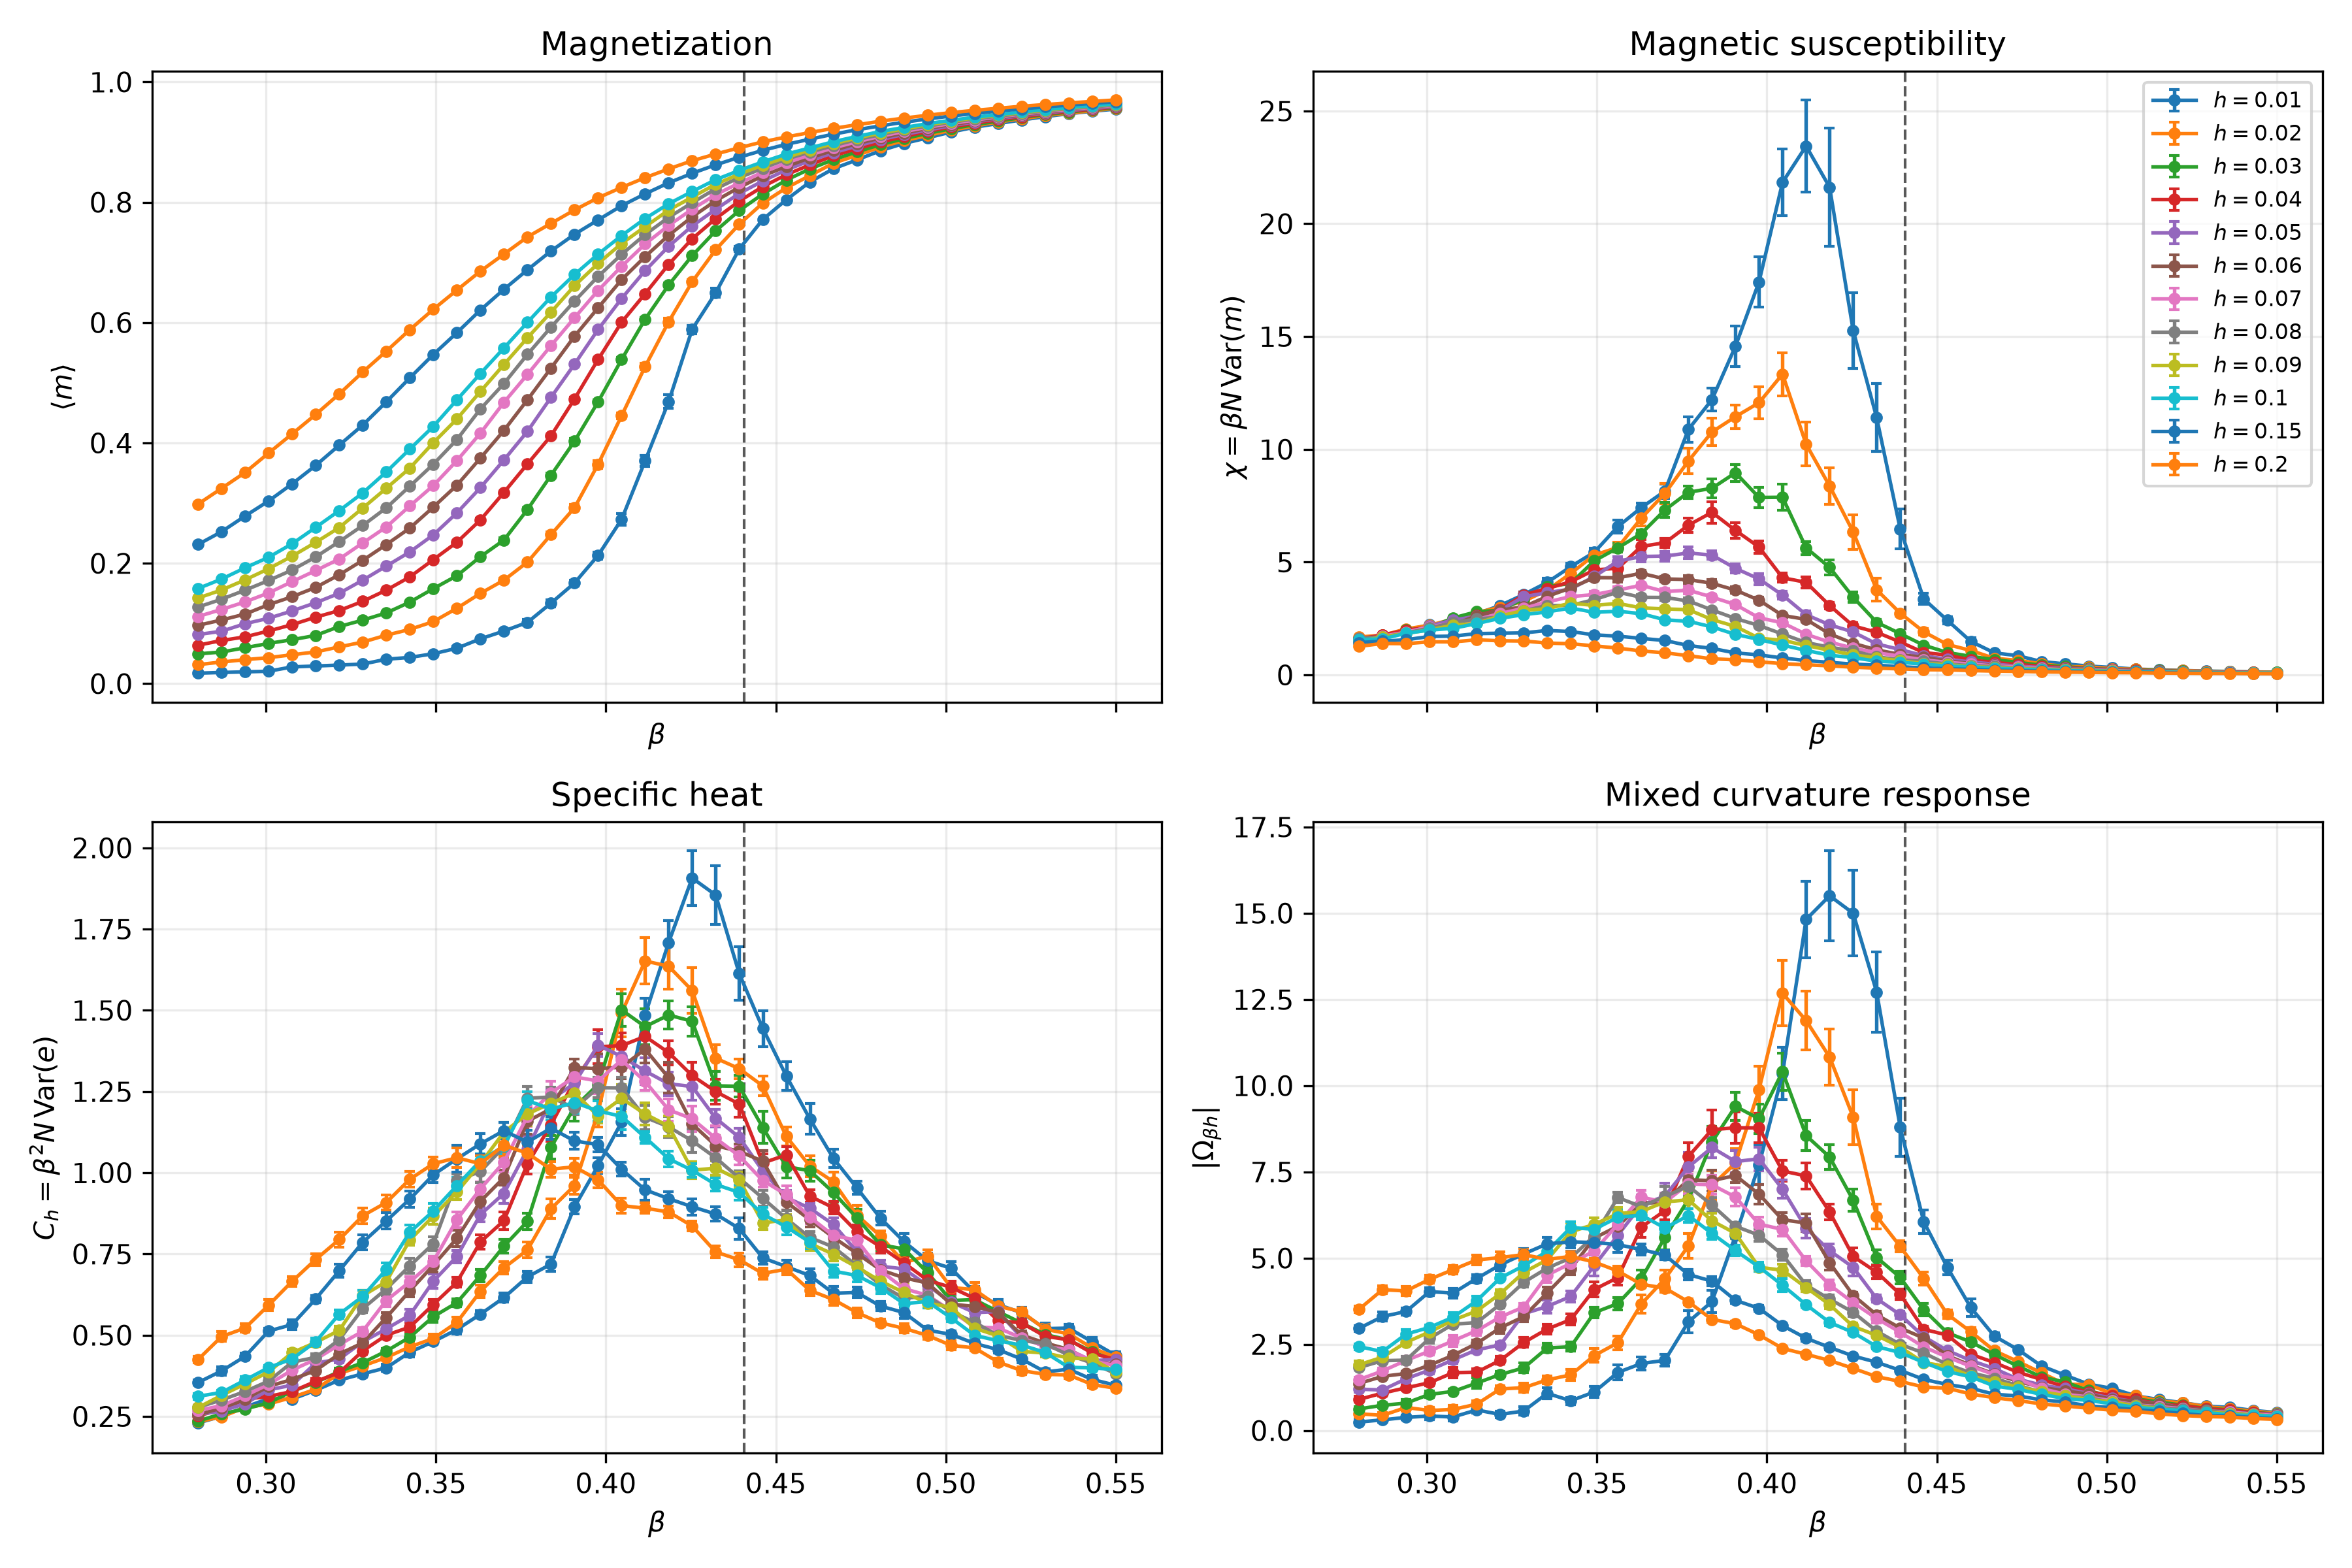
\includegraphics[width=\textwidth]{Figures/ising_cross_sections_all.png}
\caption{
Thermodynamic response functions of the two-dimensional Ising
model as functions of inverse temperature for several values
of the external magnetic field.
(a) Magnetization (m),
(b) magnetic susceptibility (\chi_T),
(c) heat capacity (C_h),
and
(d) mixed response
\(\Omega_{Th}=-\langle \delta E\delta M\rangle/(k_B T^2)\).
The first three panels represent the conventional response
functions associated with the diagonal elements of the
thermodynamic covariance matrix. The mixed response shown in
panel (d) arises from the off-diagonal covariance between
energy and magnetization fluctuations and therefore measures
the coupling between thermal and magnetic response sectors.
While all response functions exhibit enhanced behavior near the
critical region, the mixed response provides additional
information regarding the organization of correlated
fluctuations and serves as the fundamental quantity underlying
the response-geometric framework developed in this review.
}
\label{fig:ising_response_functions}
\end{figure*}
%=========================================================


Figure~\ref{fig:ising_response_functions} summarizes the
resulting response functions. Panels (a)–(c) show the
magnetization, susceptibility, and heat capacity for several
values of the external field. These quantities exhibit the
expected signatures of criticality, including enhanced response
near the Onsager critical point. Panel (d) shows the mixed
response \(\Omega_{Th}\). Although the mixed response displays
a pronounced peak near the critical region, its behavior is
qualitatively distinct from either the heat capacity or
susceptibility because it reflects the correlation between
energetic and magnetic fluctuations rather than fluctuations
within a single response sector.

At this stage it is useful to emphasize an important conceptual
shift. Conventional phase diagrams classify equilibrium states.
The quantities plotted in Fig.~\ref{fig:ising_response_functions}
instead characterize how those states respond to perturbations.
The resulting objects therefore belong naturally to a response
manifold rather than a state manifold. From this perspective,
the relevant question is no longer simply where a phase
transition occurs, but how response is distributed throughout
the surrounding thermodynamic landscape.



%=========================================================
\begin{figure*}[t]
\centering
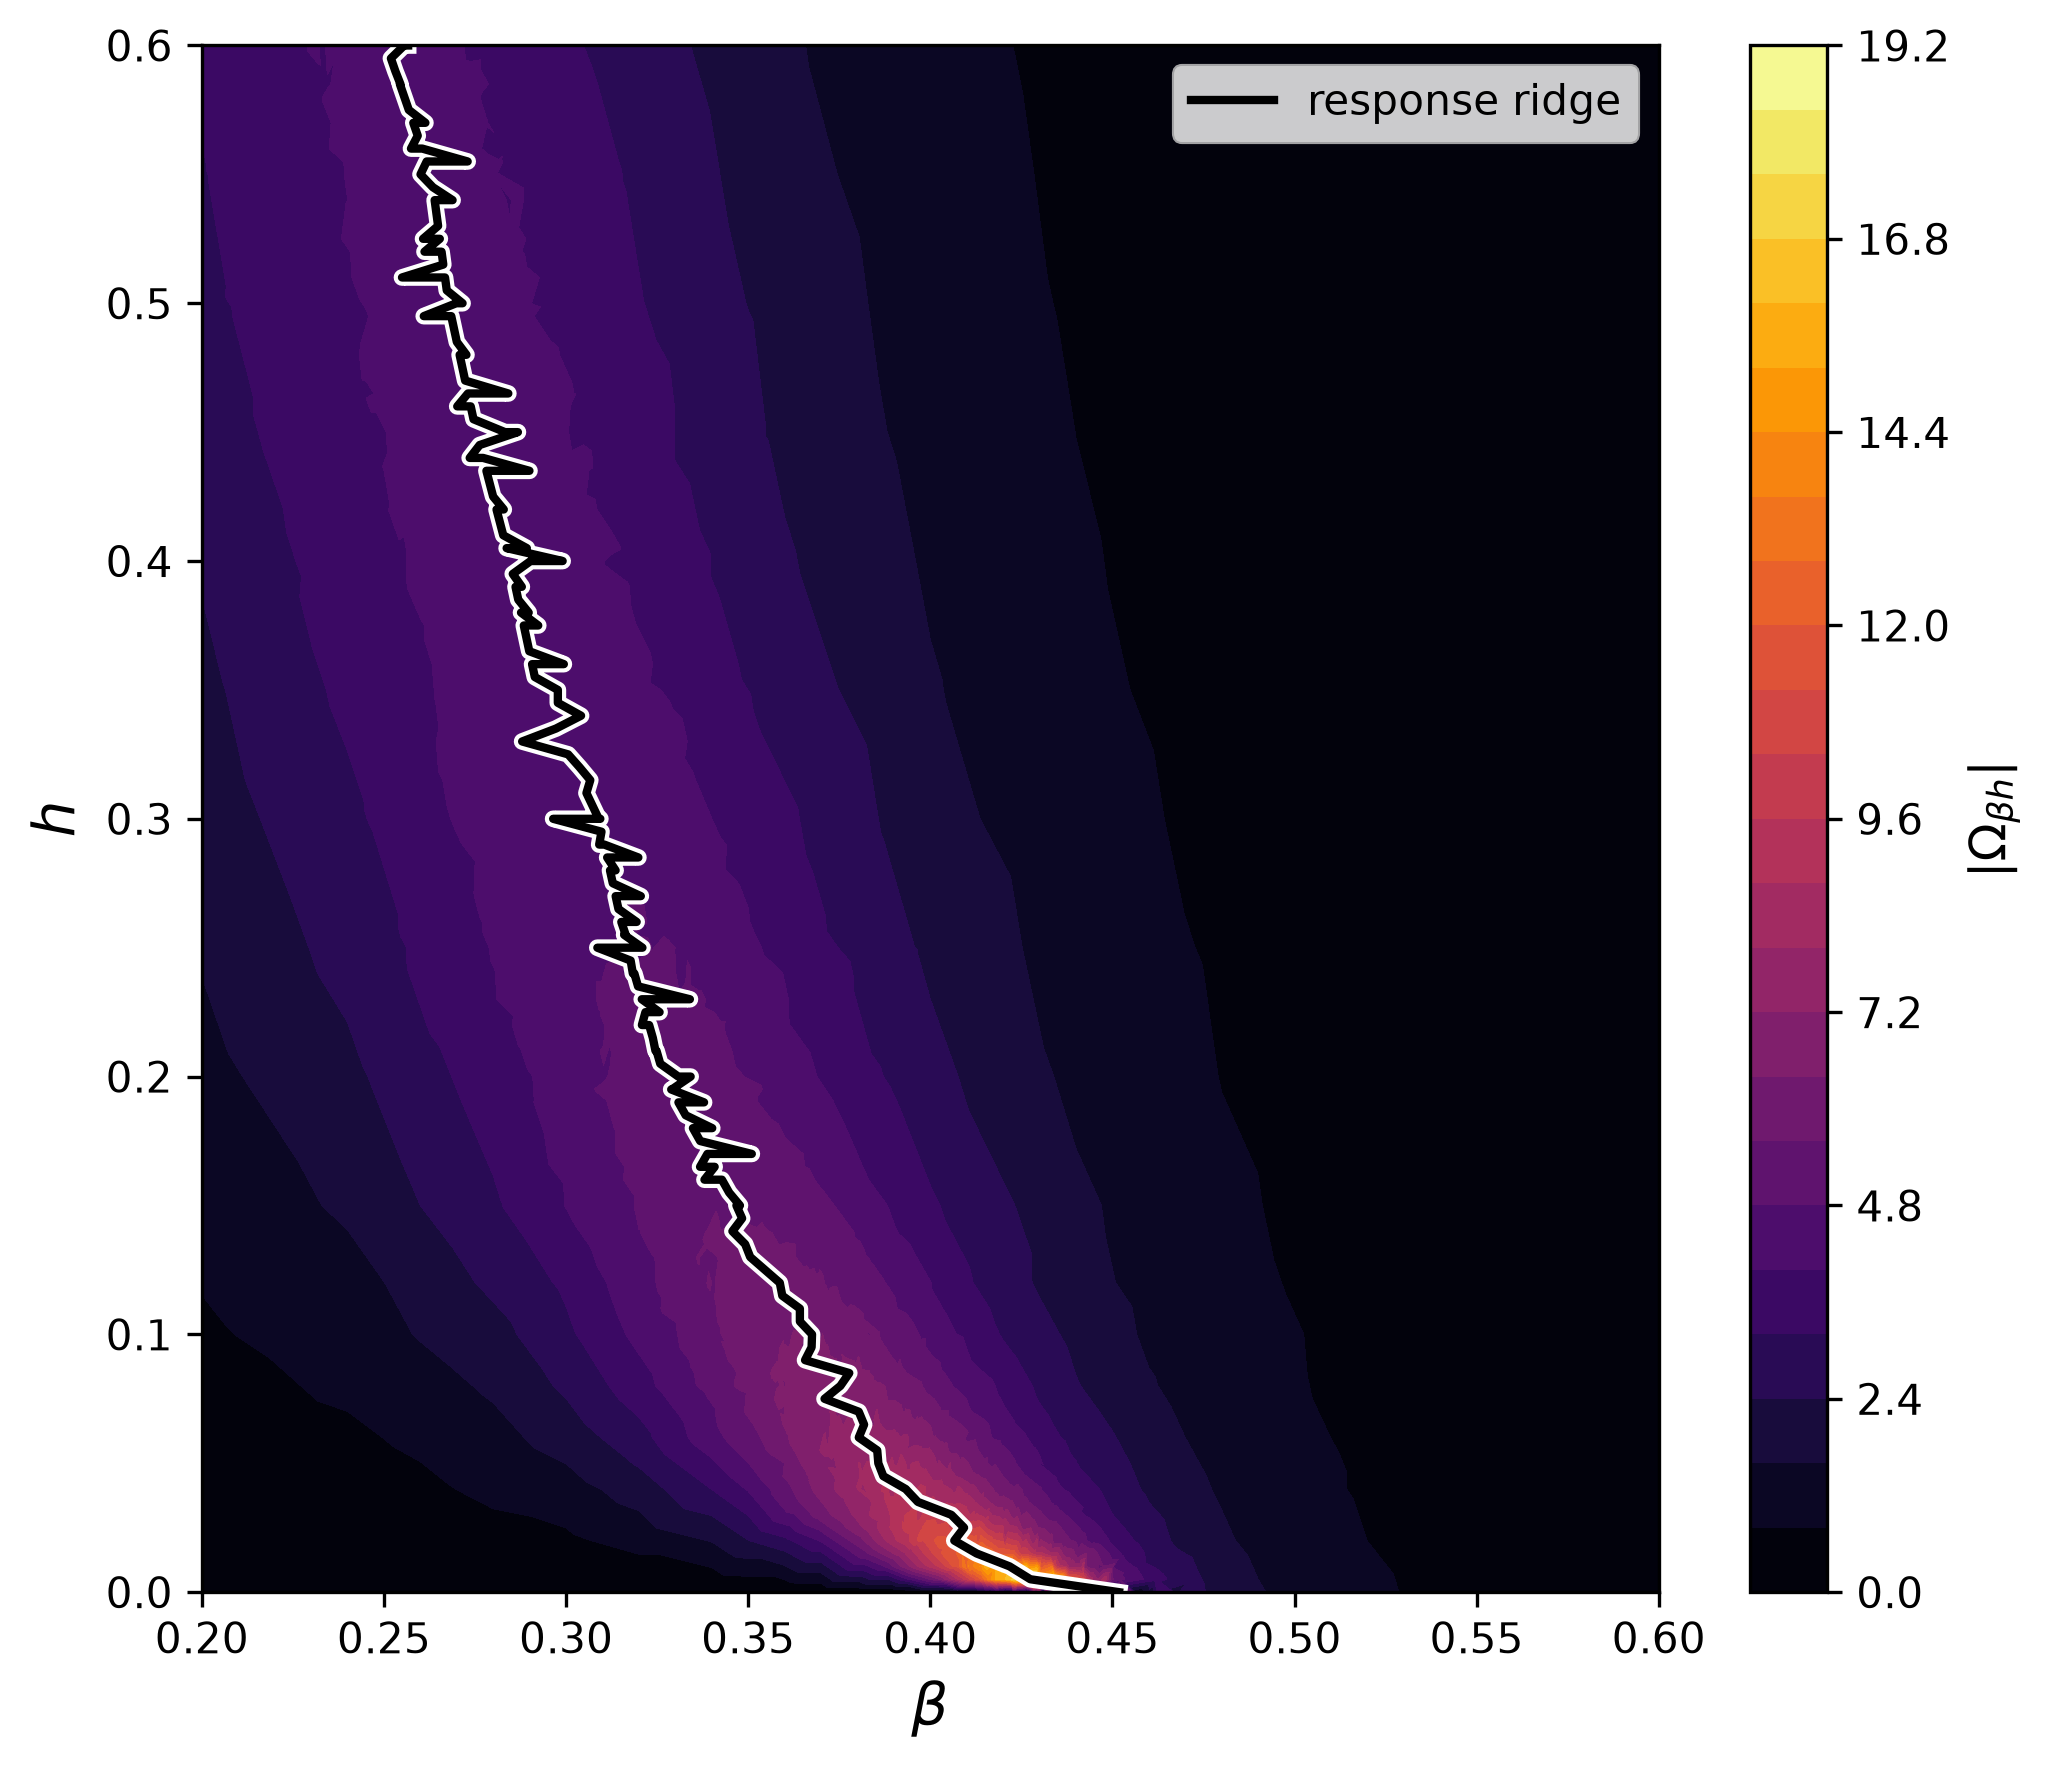
\includegraphics[width=0.85\textwidth]{Figures/ising_curvature_field_Omega.png}
\caption{
Mixed-response landscape
\(\Omega_{Th}(T,h)\)
for the two-dimensional Ising model together with the
extracted loci of maximal response.
The color scale indicates the magnitude of the mixed
fluctuation field, while the superimposed curves denote ridge
trajectories obtained from maxima of the response functions.
Unlike conventional phase diagrams, which classify equilibrium
states, the present construction characterizes how those
states respond to perturbations. The mixed-response ridge
extends well beyond the Onsager critical point into the
supercritical regime, revealing an extended pathway along
which thermal and magnetic fluctuations remain maximally
coupled. The existence of multiple ridge trajectories
associated with different response sectors demonstrates that
the supercritical region is organized by a hierarchy of
response structures rather than a single universal crossover
curve.
}
\label{fig:ising_ridge}
\end{figure*}
%=========================================================


This viewpoint becomes particularly illuminating when the mixed
response is evaluated throughout the full \((T,h)\) control
manifold. Figure~\ref{fig:ising_ridge} shows the resulting
response landscape \(\Omega_{Th}(T,h)\) together with the
extracted loci of maximal response. Rather than remaining
localized near the critical point, the mixed response organizes
into an extended ridge that persists deep into the
supercritical regime. The ridge identifies a pathway through
parameter space along which thermal and magnetic fluctuations
remain maximally coupled.

The appearance of such a structure is significant for several
reasons. First, it demonstrates that mixed fluctuations remain
organized far beyond the immediate vicinity of a thermodynamic
singularity. Second, the ridge provides a natural continuation
of collective response into the supercritical regime, where no
sharp phase boundary exists. Third, because the ridge is
constructed directly from experimentally accessible
fluctuations, it may be identified without reference to a
specific order parameter or symmetry-breaking mechanism.
Finally, the ridge reveals that phase diagrams may be viewed as
response landscapes whose geometry is encoded in the covariance
structure of the system.

An equally important result concerns the scaling behavior of the
response landscape. Analysis of the numerical data reveals that
the maxima of the heat capacity, magnetic susceptibility, and
mixed response obey distinct scaling laws as the critical
region is approached. The corresponding exponents differ,
indicating that the response matrix does not scale uniformly.
Instead, thermal, magnetic, and mixed fluctuation sectors are
amplified at different rates.

This observation admits a particularly natural geometric
interpretation. The covariance matrix defines a local
fluctuation ellipsoid whose principal axes describe the
dominant directions of thermodynamic response. If all response
sectors scaled identically, the covariance ellipsoid would
simply expand as criticality is approached. The numerical
results demonstrate that this is not the case. Because the
various response sectors exhibit distinct scaling behavior, the
covariance ellipsoid changes shape as well as size. The
response geometry therefore undergoes a continuous deformation,
with different response directions becoming dominant in
different regions of parameter space.

The loci of maximal response exhibit a similar hierarchy. The
susceptibility, heat-capacity, and mixed-response ridges follow
distinct trajectories through the control manifold, indicating
that the continuation of critical behavior into the
supercritical regime cannot be represented by a single
universal curve. Rather, the thermodynamic landscape contains a
family of response ridges associated with different fluctuation
sectors. From this perspective, the supercritical region is not
organized by a unique Widom line but by a hierarchy of response
trajectories reflecting different projections of the underlying
covariance structure.

The existence of multiple scaling sectors raises a natural
question. If the various response functions exhibit distinct
scaling behavior and define distinct ridge structures, should
they be regarded as independent coordinates of thermodynamic
response? Surprisingly, the numerical results suggest
otherwise.


%=========================================================
\begin{figure}[t]
\centering
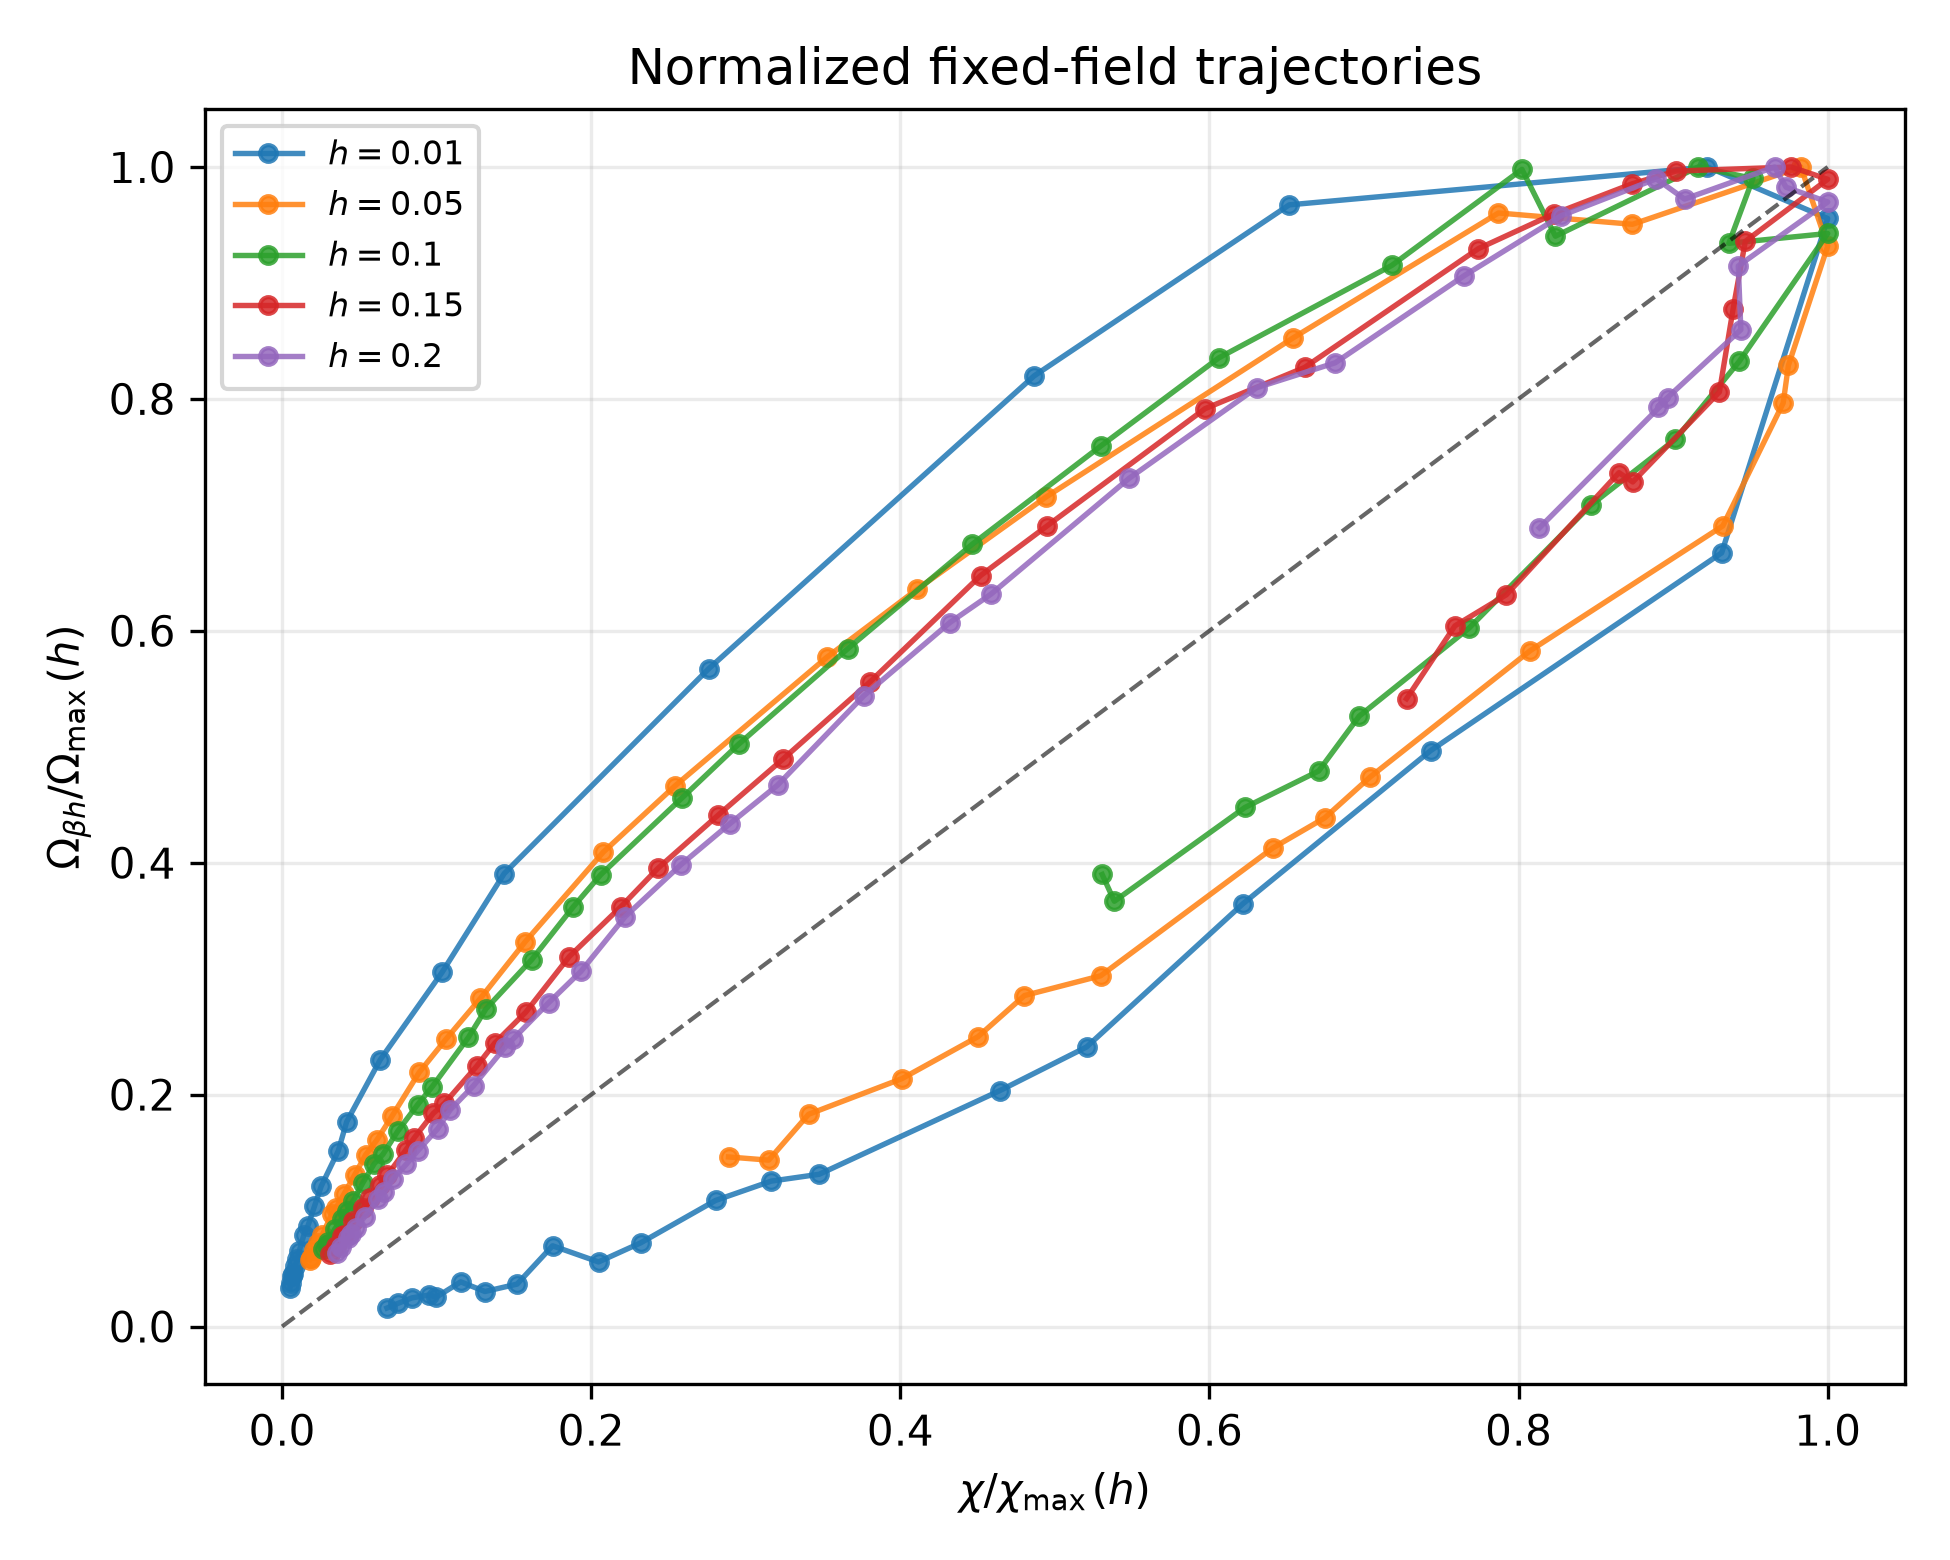
\includegraphics[width=\columnwidth]{Figures/omega_vs_chi_normalized_trajectories.png}
\caption{
Emergent response manifold in the two-dimensional Ising model.
Trajectories obtained for different values of the external
field are represented in terms of the normalized response
coordinates
\(\tilde{\chi}=\chi_T/\chi_{T,\mathrm{max}}\)
and
\(\tilde{\Omega}=\Omega_{Th}/\Omega_{Th,\mathrm{max}}\).
Despite corresponding to distinct thermodynamic trajectories
in the control manifold, the normalized responses collapse
onto an approximately universal curve. The result indicates
that the susceptibility and mixed response are not independent
observables but are constrained by an emergent geometric
relationship. The collapse provides evidence that the image of
the two-dimensional control manifold is concentrated near a
lower-dimensional object in response space, suggesting the
existence of an underlying response manifold that organizes
thermodynamic behavior across a broad range of temperatures
and fields.
}
\label{fig:response_manifold}
\end{figure}
%=========================================================

Figure~\ref{fig:response_manifold} shows representative
trajectories obtained by normalizing the response functions by
their respective maxima and representing them in response
space. Despite corresponding to different values of the
external field, the trajectories collapse onto a common curve
to a remarkable degree. The collapse suggests the existence of
an approximate functional relationship between the normalized
response variables and therefore indicates the emergence of a
low-dimensional response manifold.

The significance of this result is easily overlooked. A generic
mapping
\begin{equation}
\Phi :(T,h)
\longrightarrow (\chi_T,\Omega_{Th})
\end{equation}
from a two-dimensional control manifold into a two-dimensional
response space need not produce any collapse at all. One would
generically expect the image of the control manifold to fill a
substantial region of response space. Instead, the numerical
trajectories are concentrated near a lower-dimensional object.
The response functions therefore behave not as independent
coordinates but as quantities constrained by an emergent
geometric relationship.

Taken together, the covariance matrix, response ridges,
scaling hierarchies, and manifold collapse reveal a coherent
picture of thermodynamic response. The covariance matrix
defines the local fluctuation structure, mixed response
identifies the coupling between distinct fluctuation sectors,
the scaling hierarchy reveals the anisotropic amplification of
response, and the manifold collapse exposes a deeper geometric
constraint linking apparently independent observables.
Geometry therefore emerges not from the equilibrium states
themselves but from the organization of response. The Ising
model thus provides a concrete demonstration of the central
theme of this review: geometric structure is encoded not only
in states, but in how those states respond to external
perturbations.



\subsection{Response Geometry from Thermodynamic Potentials: Spin–Peierls and Orbital Models}

The Ising model provides perhaps the simplest realization of
response geometry, demonstrating that thermodynamic metrics and
mixed response functions may be reconstructed directly from
equilibrium fluctuations. More generally, however, many quantum
materials are described by microscopic Hamiltonians from which an
effective thermodynamic potential may be constructed explicitly.
This raises an important question: are the geometric structures
identified through statistical fluctuations peculiar to the
Ising model, or do they represent more general features of
thermodynamic response?

An ideal setting in which to address this question is provided
by spin–Peierls and related orbital models. These systems
occupy a central position in condensed-matter physics because
they naturally couple spin, orbital, electronic, and lattice
degrees of freedom through a dimerization instability. Their
importance extends well beyond the original description of
quasi-one-dimensional magnetic materials. Closely related
Hamiltonians underlie the Su–Schrieffer–Heeger (SSH) model of
conducting polymers, one-dimensional topological insulators,
correlated transition-metal oxides, synthetic quantum lattices,
photonic crystals, superconducting circuits, and other
engineered quantum materials. Although these systems are often
discussed from the perspective of topological band theory and
Berry phases, they also provide a rich arena for exploring the
geometry of thermodynamic response.

The conceptual distinction is an important one. Berry geometry
describes the evolution of quantum eigenstates under adiabatic
parameter variation, whereas the framework developed here is
concerned with the geometry of thermodynamic observables. The
relevant mathematical object is therefore not the wavefunction
or Bloch eigenstate, but the thermodynamic potential from which
the observable response is derived. This shift in perspective
allows the same microscopic Hamiltonian to be viewed through the
lens of equilibrium fluctuations, response functions, and
thermodynamic geometry.

Unlike the Ising model, where the response matrix was
reconstructed numerically from Monte Carlo covariances, the
models considered here admit an explicit microscopic
Hamiltonian. The thermodynamic response is obtained by
constructing the partition function and the corresponding
free-energy functional, from which all response quantities
follow by differentiation. As we shall show, this entirely
different computational route leads to remarkably similar
response landscapes, suggesting that the geometric structures
identified in the previous section are intrinsic properties of
thermodynamic response rather than artifacts of a particular
numerical methodology.

As a representative example, we consider the spin–Peierls
compound \ce{CuGeO3}, whose coupled spin, orbital, and lattice
degrees of freedom provide a realistic platform for illustrating
how response geometry emerges directly from a microscopic
Hamiltonian. In addition to its relevance for equilibrium
thermodynamics, the same Hamiltonian forms the starting point
for the nonequilibrium and spectroscopic developments discussed
in later sections, providing a direct bridge between
thermodynamic response, open quantum systems, and nonlinear
optical spectroscopy.


\subsubsection{Microscopic Spin–Orbital Hamiltonian}

To illustrate the construction of response geometry from a
microscopic theory, we consider a generic spin–orbital lattice
model representative of spin–Peierls materials such as
\ce{CuGeO3}. Rather than beginning from a phenomenological
Landau free-energy functional, we adopt a Hamiltonian that
explicitly incorporates the coupled spin, orbital, and lattice
degrees of freedom responsible for the thermodynamic response.
This formulation is sufficiently general to encompass not only
spin–Peierls compounds, but also the broader class of
Su–Schrieffer–Heeger (SSH) and dimerized lattice models that
appear throughout condensed-matter physics.

The microscopic Hamiltonian is written as
\begin{align}
H=H_{\mathrm{spin}}+H_{\mathrm{orb}}+H_{\mathrm{SO}}+H_{\mathrm{ph}}
+
H_{\mathrm{sp-ph}},
\end{align}
where the individual contributions describe magnetic exchange,
orbital energetics, spin–orbit coupling, lattice vibrations,
and spin–phonon interactions, respectively.

The magnetic degrees of freedom are described by an
antiferromagnetic Heisenberg chain,
\begin{align}
H_{\mathrm{spin}}
=
\sum_i
J_i(B,T),
\mathbf{S}i\cdot\mathbf{S}{i+1}
+
g\mu_BB
\sum_i
S_i^z,
\end{align}
where the nearest-neighbor exchange interaction is modulated by
the spin–Peierls distortion,
\begin{align}
J_i(B,T) =
J_0 + (-1)^i\delta(B,T).    
\end{align}

Unlike a conventional lattice parameter, the dimerization
amplitude \(\delta(B,T)\) is not fixed. Instead, it is an
emergent thermodynamic field determined self-consistently by
minimizing the equilibrium free-energy functional. As the
temperature and magnetic field vary, the equilibrium lattice
distortion evolves continuously over the thermodynamic control
manifold, modifying the exchange interaction and, consequently,
the magnetic excitation spectrum. The microscopic Hamiltonian
therefore depends implicitly upon the external control
variables through the equilibrium order parameter
\(\delta(B,T)\).

The orbital Hamiltonian describes the crystal-field splitting of
the \ce{Cu^{2+}} \ce{3d^9} manifold within the elongated
$D_{4h}$ ligand environment,
\begin{align}
H_{\mathrm{orb}}
=
\sum_{i,\alpha}
\epsilon_\alpha
n_{i\alpha},
\end{align}
while the spin–orbit interaction,
\begin{align}
H_{\mathrm{SO}}
=
\lambda
\sum_i
\mathbf{L}_i\cdot\mathbf{S}_i,
\end{align}
couples the spin and orbital sectors. Together with the lattice
Hamiltonian and the spin–phonon interaction, these terms
produce a microscopic description in which spin, orbital, and
structural degrees of freedom evolve cooperatively under the
influence of temperature and magnetic field.

Although the real-space representation most clearly exposes the
physical origin of the competing interactions, it is often
convenient to transform to reciprocal space. Introducing the
Fourier-transformed operators,
\begin{align}
c_{i\alpha}
=
\frac{1}{\sqrt{N}}
\sum_k
e^{ikR_i}
c_{k\alpha},
\end{align}
the Hamiltonian becomes
\begin{align}
H
=
\sum_k
\Psi_k^\dagger
\mathcal{H}(k;\delta(B,T))
\Psi_k,
\end{align}
where the Bloch Hamiltonian contains the dimerized exchange,
crystal-field splitting, and spin–orbit coupling in a form
closely analogous to the SSH model. In this representation, the
spin–Peierls distortion opens a gap at the Brillouin-zone
boundary while simultaneously modifying the spin and orbital
character of the low-energy quasiparticles.

This momentum-space representation provides the natural
starting point for constructing the partition function and the
equilibrium free-energy functional. More importantly, it
illustrates that the Hamiltonian is not merely parameterized by
the external thermodynamic variables but is itself reshaped by
the equilibrium order parameter \(\delta(B,T)\). The response
geometry developed below therefore reflects both the explicit
dependence of the free energy on the thermodynamic control
variables and the implicit evolution of the microscopic
Hamiltonian through the self-consistent lattice distortion.

\subsubsection{From the Spin--Orbital Hamiltonian to a Free-Energy Functional}
The self-consistent nature of the spin--Peierls distortion makes
the construction of the thermodynamic potential especially
important. The Hamiltonian depends on the external control
variables both explicitly, through the Zeeman coupling to the
magnetic field, and implicitly through the equilibrium
dimerization amplitude \(\delta(T,h)\). The response geometry
therefore cannot be obtained by differentiating microscopic
Hamiltonian parameters alone. Instead, it emerges only after the
equilibrium thermodynamic potential has been constructed.
For a fixed value of the dimerization amplitude, the
momentum-space Hamiltonian defines the partition function
\begin{align}
Z(T,h;\delta)
=
\mathrm{Tr}
\exp\!\left[
-\beta H(h;\delta)
\right].
\end{align}
In the band representation this may be written as
\begin{align}
Z(T,h;\delta)
=
\prod_{k,n}
\left[
1+
\exp\!\left(
-\beta\varepsilon_n(k;h,\delta)
\right)
\right],
\end{align}
where \(\varepsilon_n(k;h,\delta)\) denotes the eigenvalues of
the Bloch Hamiltonian
\(\mathcal{H}(k;h,\delta)\).
The corresponding electronic contribution to the free energy is
\begin{align}
F_{\rm el}(T,h;\delta)
=
-k_BT
\sum_{k,n}
\ln\!\left[
1+
\exp\!\left(
-\beta\varepsilon_n(k;h,\delta)
\right)
\right].
\end{align}
The total free energy contains both the electronic and elastic
contributions,
\begin{align}
F(T,h;\delta)
=
F_{\rm el}(T,h;\delta)
+
\frac{K}{2}\delta^2
+
F_{\rm ph}(T),
\end{align}
where \(K\) is the effective stiffness of the Peierls mode and
\(F_{\rm ph}\) denotes the remaining phonon contribution.
The equilibrium dimerization is determined by minimizing the
free energy at each point of the thermodynamic control manifold,
\begin{align}
\left.
\frac{\partial F(T,h;\delta)}
{\partial\delta}
\right|_{\delta=\delta_\ast(T,h)}
=
0,
\end{align}
so that
\begin{align}
\delta(T,h)
=
\delta_\ast(T,h).
\end{align}
The free-energy minimization therefore defines the mapping
\[
(T,h)
\longrightarrow
\delta_\ast(T,h),
\]
so that the equilibrium order parameter becomes an emergent
field over the thermodynamic control manifold.
The physical thermodynamic potential is consequently
\begin{align}
F_{\rm eq}(T,h)
=
F\!\left(T,h;\delta_\ast(T,h)\right).
\end{align}
This distinction is essential. The response functions are not
obtained by holding the microscopic dimerization fixed, but by
differentiating the equilibrium free energy after the order
parameter has been determined self-consistently. Consequently,
the thermodynamic derivatives contain both explicit derivatives
with respect to the external control variables and implicit
contributions arising from the evolution of
\(\delta_\ast(T,h)\).
Because \(F_{\rm eq}(T,h)\) is a thermodynamic state function,
its differential is exact,
\begin{align}
dF_{\rm eq}
=
-S\,dT
-
m\,dh.
\end{align}
The entropy and magnetization follow immediately from
\begin{align}
S
&=
-
\left(
\frac{\partial F_{\rm eq}}
{\partial T}
\right)_h,
\\
m
&=
-
\left(
\frac{\partial F_{\rm eq}}
{\partial h}
\right)_T.
\end{align}
The second derivatives define the thermodynamic response
functions,
\begin{align}
C_h
&= - T
\left(
\frac{\partial^2F_{\rm eq}}
{\partial T^2}
\right)_h,
\\
\chi_T
&=
-\left(
\frac{\partial^2F_{\rm eq}}
{\partial h^2}
\right)_T,
\\
\Omega_{Th}
&=
-
\frac{\partial^2F_{\rm eq}}
{\partial T\,\partial h}
=
-
\left(
\frac{\partial m}{\partial T}
\right)_h
=
-
\left(
\frac{\partial S}{\partial h}
\right)_T.
\end{align}
Since the numerical calculations are performed in terms of the
inverse temperature,
\(\beta=(k_BT)^{-1}\),
the response maps presented below are expressed as
\begin{align}
\Omega_{\beta h}
=
\left(
\frac{\partial m}
{\partial\beta}
\right)_h,
\end{align}
which differs from \(\Omega_{Th}\) only through the Jacobian
relating derivatives with respect to \(T\) and \(\beta\).
This is the quantity shown in
Fig.~\ref{fig:cugeo3_response}.

The construction developed here illustrates an important
principle that extends well beyond the specific spin--Peierls
model. The response geometry is not inherited directly from the
microscopic Hamiltonian, but from the thermodynamic potential
constructed from that Hamiltonian. The role of the microscopic
model is to define the statistical ensemble and, through the
partition function, the equilibrium free-energy functional.
Once the equilibrium order parameter has been determined
self-consistently, the exact differential of the resulting
thermodynamic potential generates the complete response
structure through its first and second derivatives.
In the present model, the spin--Peierls order parameter
\(\delta_\ast(T,h)\) serves as an emergent thermodynamic field
defined over the control manifold. The microscopic Hamiltonian
therefore depends implicitly upon the thermodynamic state,
reflecting the self-consistent evolution of the equilibrium
lattice distortion. Consequently, the response functions encode
not only the explicit dependence of the free energy on the
external control variables, but also the collective
reorganization of the underlying spin, orbital, and lattice
degrees of freedom.

This distinction is central to the geometric framework developed
throughout this review. Different physical systems may employ
very different microscopic Hamiltonians and computational
methods---Monte Carlo sampling in the Ising model,
self-consistent free-energy minimization in the spin--Peierls
model, or nonequilibrium steady-state density matrices in open
quantum systems. Nevertheless, the geometric objects themselves
always derive from the thermodynamic or dynamical response
rather than from the microscopic representation used to compute
it. Response geometry is therefore a property of the response
manifold, not of the Hamiltonian from which that response is
obtained.
\begin{figure*}[t]
\centering
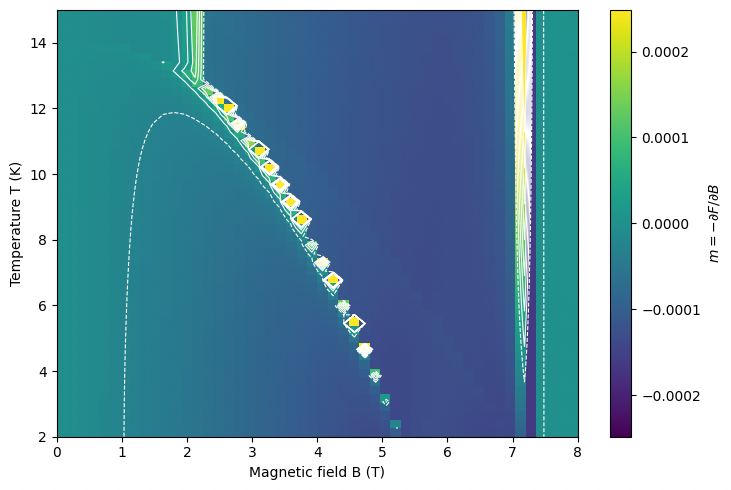
\includegraphics[width=0.48\textwidth]{Figures/CuGeO3-mag.png}
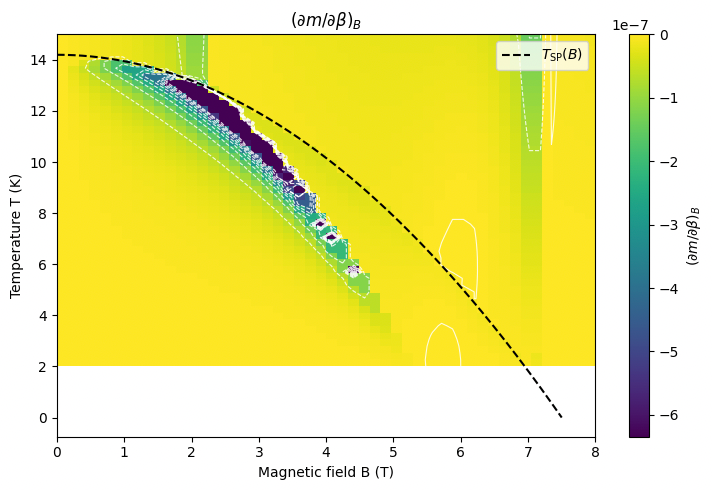
\includegraphics[width=0.48\textwidth]{Figures/CuGeO3-mixed-deriv.png}
\caption{
Response geometry of the spin--Peierls model for \ce{CuGeO3}.
(a) Magnetization landscape \(\langle m\rangle(B,T)\) over the
magnetic-field--temperature control manifold.
(b) Mixed thermal-field response
\((\partial m/\partial \beta)_B\), obtained by differentiating
the free-energy functional. The dashed curve denotes the
spin--Peierls transition scale \(T_{\rm SP}(B)\). The mixed
response develops an extended ridge that tracks the reorganization
of the spin--Peierls state under magnetic field. Unlike the Ising
case, where the response geometry is reconstructed from Monte Carlo
covariances, here the same geometric structure is obtained directly
from a thermodynamic potential.
}
\label{fig:cugeo3_response}
\end{figure*}

\subsection{Rewrite: Phenomenological Spin--Peierls Model for \ce{CuGeO3}}
As a second example of equilibrium response geometry, we consider
a phenomenological spin--Peierls model motivated by \ce{CuGeO3}.
Unlike the Ising model, where the response functions were obtained
from Monte Carlo sampling of equilibrium fluctuations, the present
calculation proceeds by constructing a microscopic free-energy model
and differentiating the resulting thermodynamic potential. This
provides a complementary route to response geometry: the response
manifold is generated not from sampled covariances, but from a
field- and temperature-dependent free-energy landscape.

The model combines an SSH-like orbital band Hamiltonian with a
phenomenological spin--Peierls order parameter. The total free energy
is written as
\begin{align}
F(T,B)
=
F_{\rm band}(T,B)
+
F_{\rm spin}(T,B)
+
F_{\rm SP}(T,B).
\end{align}
The band contribution is obtained from a two-sublattice Bloch
Hamiltonian with five real \(d\)-orbitals,
\[
(d_{xy},d_{yz},d_{xz},d_{x^2-y^2},d_{z^2}),
\]
including ligand-field splittings, spin--orbit coupling, Zeeman
coupling, and an SSH-like hopping alternation. The local Hamiltonian
has the form
\begin{align}
H_{\rm loc}
=
H_{\rm lf}
+
\lambda_{\rm SO}\,\mathbf L\cdot\mathbf S
+
\mu_B
\left(
k_{\rm orb}\mathbf L
+
g_s\mathbf S
\right)\cdot\mathbf B,
\end{align}
where the orbital angular momentum matrices are represented in the
real \(d\)-orbital basis.
The Bloch Hamiltonian is defined on a two-sublattice unit cell as
\begin{align}
\mathcal H(k)
=
\begin{pmatrix}
H_{\rm loc} & Q(k)\\
Q^\dagger(k) & H_{\rm loc}
\end{pmatrix},
\end{align}
with
\begin{align}
Q(k)
=
T_1+T_2 e^{-ik},
\qquad
T_1=(1+\delta)T_0,
\qquad
T_2=(1-\delta)T_0.
\end{align}
Here \(T_0\) contains orbital-diagonal hopping amplitudes and selected
inter-orbital hopping terms. The hopping dimerization is tied to the
spin--Peierls order parameter through
\begin{align}
\delta_t(T,B)
=
\delta_{t0}\,\phi(T,B).
\end{align}
For eigenvalues \(\varepsilon_n(k)\) of \(\mathcal H(k)\), the band
free energy is evaluated as
\begin{align}
F_{\rm band}
=
-\frac{1}{\beta}
\frac{1}{N_k}
\sum_{k,n}
\ln
\left[
1+
\exp\left(-\beta \varepsilon_n(k)\right)
\right].
\end{align}
The spin--Peierls order parameter is introduced phenomenologically
using a mean-field field-dependent transition temperature,
\begin{align}
T_{\rm SP}(B)
=
T_{\rm SP}^{0}
\left[
1-\left(\frac{B}{B_c}\right)^2
\right],
\end{align}
and
\begin{align}
\phi(T,B)
=
\sqrt{1-\frac{T}{T_{\rm SP}(B)}}
\sqrt{1-\left(\frac{B}{B_c}\right)^2},
\end{align}
for \(T<T_{\rm SP}(B)\) and \(|B|<B_c\), with
\(\phi(T,B)=0\) otherwise. The corresponding spin--Peierls gap is
\begin{align}
\Delta_{\rm SP}(T,B)
=
\Delta_{\rm SP}^{0}\phi(T,B).
\end{align}
The spin excitation spectrum is modeled by
\begin{align}
E_0(k)
=
\sqrt{
\Delta_{\rm SP}^2
+
\epsilon_k^2
},
\qquad
\epsilon_k
=
J_1\cos k+J_2\cos(2k),
\end{align}
with Zeeman-shifted branches
\begin{align}
E_{\pm}(k)
=
E_0(k)
\pm
g_s\mu_B B.
\end{align}
The spin contribution to the free energy is then
\begin{align}
F_{\rm spin}
=
\frac{1}{\beta}
\frac{1}{N_k}
\sum_k
\left[
\ln\left(1-e^{-\beta E_+(k)}\right)
+
\ln\left(1-e^{-\beta E_-(k)}\right)
\right].
\end{align}
Finally, a Landau-like stabilization term is included,
\begin{align}
F_{\rm SP}
=
-K_{\rm SP}
\left(\Delta_{\rm SP}^{0}\right)^2
\phi^2(T,B),
\end{align}
which favors the ordered spin--Peierls state below the transition
line.

The thermodynamic response functions are obtained by numerical
differentiation of the resulting free energy. The magnetization proxy
is
\begin{align}
m(T,B)
=
-
\left(
\frac{\partial F}{\partial B}
\right)_T,
\end{align}
and the mixed thermal-field response is
\begin{align}
R_\beta(T,B)
=
\left(
\frac{\partial m}{\partial\beta}
\right)_B.
\end{align}
This is the response field plotted in
Fig.~\ref{fig:cugeo3_response}. We also compute the magnetic
susceptibility proxy
\begin{align}
\chi_B(T,B)
=
\left(
\frac{\partial m}{\partial B}
\right)_T.
\end{align}
A Widom-line-like crossover ridge is extracted by locating, at each
fixed magnetic field, the temperature where the magnitude of the
mixed response is maximal,
\begin{align}
T^\ast(B)
=
\operatorname*{arg\,max}_{T}
\left|
R_\beta(T,B)
\right|.
\end{align}
The present calculation should be interpreted as a phenomenological
spin--Peierls response model rather than a fully self-consistent
minimization over the lattice distortion. The order parameter
\(\phi(T,B)\) is specified by the mean-field ansatz above and then
used to construct the band, spin, and Landau contributions to the
free energy. The response geometry is inherited from the resulting
thermodynamic potential \(F(T,B)\). Thus, as in the Ising model, the
geometric quantities are properties of the response manifold, not of
the microscopic Hamiltonian alone.


\subsection{Summary}
The examples considered in this section demonstrate that response geometry is independent of the computational framework used to obtain the thermodynamic potential. Whether reconstructed from equilibrium fluctuations or derived analytically from a microscopic free-energy functional, the same geometric structures emerge from the response manifold. This observation naturally raises the question of whether an analogous construction exists for systems that possess no equilibrium thermodynamic potential. The answer, developed in the following sections, is affirmative. In open quantum systems the free energy is replaced by the nonequilibrium steady-state density operator, and the exact differential of equilibrium thermodynamics gives way to a response one-form whose non-exactness generates an intrinsic curvature. The resulting framework may therefore be viewed as the quantum generalization of response geometry developed here.


